%
% File acl2017.tex
%
%% Based on the style files for ACL-2015, with some improvements
%%  taken from the NAACL-2016 style
%% Based on the style files for ACL-2014, which were, in turn,
%% based on ACL-2013, ACL-2012, ACL-2011, ACL-2010, ACL-IJCNLP-2009,
%% EACL-2009, IJCNLP-2008...
%% Based on the style files for EACL 2006 by 
%%e.agirre@ehu.es or Sergi.Balari@uab.es
%% and that of ACL 08 by Joakim Nivre and Noah Smith

\documentclass[11pt,a4paper]{article}
\usepackage[hyperref]{acl2017}
\usepackage{times}
\usepackage{latexsym}
\usepackage{xcolor}
\usepackage[normalem]{ulem}
\usepackage{url}
\usepackage{caption}
\usepackage{subcaption}
\usepackage{pgfplots}
\usepackage{tikz}

\definecolor{forestgreen}{rgb}{0.13, 0.55, 0.13}

% Define bar chart colors
%
\definecolor{bblue}{HTML}{4F81BD}
\definecolor{rred}{HTML}{C0504D}
\definecolor{ggreen}{HTML}{9BBB59}
\definecolor{ppurple}{HTML}{9F4C7C}

%\aclfinalcopy % Uncomment this line for the final submission
%\def\aclpaperid{***} %  Enter the acl Paper ID here

%\setlength\titlebox{5cm}
% You can expand the titlebox if you need extra space
% to show all the authors. Please do not make the titlebox
% smaller than 5cm (the original size); we will check this
% in the camera-ready version and ask you to change it back.

\newcommand\BibTeX{B{\sc ib}\TeX}

% Writing macros
\newcommand{\secref}[1]{Section~\ref{ssec:#1}}
\newcommand{\figref}[1]{Figure~\ref{#1}}
\newcommand{\tabref}[1]{Table~\ref{#1}}
\newcommand{\isection}[2]{\section{#1}\label{ssec:#2}}
\newcommand{\isectionb}[1]{\section{#1}\label{ssec:#1}}
\newcommand{\com}[1]{}

% Editing macros
\newcommand{\my}[1]{\footnote{\color{red}{\textbf{#1}}}}

\newcommand{\ms}[1]{{\color{cyan}\{\textit{#1}\}$_{ms}$}}
\newcommand{\roy}[1]{\footnote{\color{red}{\textbf{Roy: #1}}}}
\newcommand{\royb}[2]{{\color{red}{\sout{#1}}}{\color{green}{#2}}}
\newcommand{\royc}[3]{\royb{#1}{#2}\roy{#3}}
\newcommand{\yc}[1]{{\color{bblue}\{\textit{#1}\}$_{yc}$}}

%\renewcommand{\ms}[1]{}
%\renewcommand{\roy}[1]{}
%\renewcommand{\royb}[1]{}
%\renewcommand{\royc}[1]{}


\title{The Effect of Different Writing Tasks on Linguistic Style:\\ A Case Study of the ROC Story Cloze Task}

\author{First Author \\
  Affiliation / Address line 1 \\
  Affiliation / Address line 2 \\
  Affiliation / Address line 3 \\
  {\tt email@domain} \\\And
  Second Author \\
  Affiliation / Address line 1 \\
  Affiliation / Address line 2 \\
  Affiliation / Address line 3 \\
  {\tt email@domain} \\}

\date{}

\begin{document}
\maketitle
\begin{abstract}
%People's writing style is affected by many factors, including topics, sentiment, and individual personality. 
People's writing style depends not just on the authors' personal traits but also on the intent and the cognitive states of the authors. 
%In this paper we show that engaging authors in different  writing tasks results in them adopting different writing styles.
In this paper, we show how similar writing tasks involving different cognitive processes can lead to measurable differences in people's writing style. % of the same authors.  
%As a case study, we experiment with a recently published machine reading task: 
We present a case study based on 
the  {\it story cloze task} \cite{Mostafazadeh:2016}, %.
%In this task, annotators were asked to generate two sentences: one which makes sense given a previous paragraph and another which doesn't.
where annotators were assigned with similar writing tasks with different constraints: (1) writing an entire story on their own vs. adding only a story ending for a given story context and (2) writing a story ending that makes the overall story coherent vs. incoherent. 
%We show that a linear classifier, which applies only simple style features, such as sentence length and character n-grams, 
We show that a simple linear classifier informed with stylistic features obtains 
state-of-the-art results on the story cloze challenge,
substantially higher than sophisticated deep learning models,
even without looking at the story context. 
%Importantly, our model doesn't even look at the previous paragraph, just the two candidate sentences, which, out of context, differ only in the writing task presented to the authors. 
Our results demonstrate that different task framings can dramatically affect the way people write. 
They also provide important lessons for designing new NLP tasks.

\end{abstract}

\section{Introduction}
Writing style is 
%defined as the the author's choice of words, spelling, grammar and punctuation.\footnote{\url{https://en.wikipedia.org/wiki/Writing_style}}
expressed through a range of linguistic elements such as words, sentence structure, and rhetorical devices.
%It is often affected by inter-writer 
It is influenced by both 
personal 
factors such as age \cite{Schler:2006}, gender \cite{Argamon:2003} 
%or mere 
and 
personality \cite{Stamatatos:2009}, 
%but also by other parameters 
and the cognitive states of the authors such as 
%such as the sentiment of the text \cite{Davidov:2010}, its level of sarcasm \cite{Tsur:2010} and whether it's deceptive \cite{Feng:2012}.
sentiment \cite{Davidov:2010}, sarcasm \cite{Tsur:2010}, and deception \cite{Feng:2012}.  
In this paper, we study 
%to what extent is 
the extent to which people's 
writing style is affected by intricate factors, such as 
the nature of the writing task that would involve different cognitive processes. 

\begin{table}[!t]
%\small
\begin{tabular}{|p{1.6cm}|p{5.3cm}|} \hline
{\bf Type} & {\bf Example} \\ \hline
{\color{blue}{\it Original}} story & My mother loves clocks that chime.	Her house is full of them.	She sets them each a little different so she can hear them chime.	It sounds like a bell tower during a wedding in her house all day.	{\color{blue}{When I visit I stop them or I'd never be able to sleep at night.}} \\ \hline
{\color{forestgreen}{\it Coherent}} story & Kathy went shopping.	She found a pair of great shoes.	The shoes were \$300.	She bought the shoes.	{\color{forestgreen}{She felt buyer's remorse after the purchase.}} \\ \hline
{\color{red}{\it Incoherent}} story & Kathy went shopping.	She found a pair of great shoes.	The shoes were \$300.	She bought the shoes.	{\color{red}{Kathy hated buying shoes.}} \\ \hline
\end{tabular}
\caption{\label{ROC-example}
Examples of stories from the story cloze task. The first row shows an {\it original} story written by one author. 
The second and third row show revised stories with two contrastive endings:
 %of the same story: 
 a {\it right} ending and a {\it wrong} one.
}
%\end{center}
\end{table}


%As a testbed, we experiment with
As a case study, we present experiments   based on 
the recently introduced ROC story cloze task \cite{Mostafazadeh:2016}. 
In this task, crowdsourced authors were asked to write five-sentence self-contained stories, henceforth {\it original} stories.
%Following, 
Then, 
%the stories were given to other authors, 
each original story was given to a different author, 
who was shown only the first four sentences as a story context, 
and asked to write contrastive story endings: a {\it right} (coherent) ending, and a {\it wrong} (incoherent) ending. 
%The goal of the task is to determine which of the endings is the correct one.
Framed as a story cloze task, the goal of this dataset was to serve as a commonsense challenge. 
\tabref{ROC-example} shows an example of an {\it original} story, a {\it coherent} story and an {\it incoherent} story.

While originally designed to be 
%a machine reading task, 
a commonsense story understanding challenge, 
%the compilation of this task 
the annotation process  
%raises several research questions
triggers interesting questions 
%which seem to differ from the original intent of the designers.
that may go beyond the original intent of the designers.
First, do 
%authors use different
people maintain the same writing 
style when asked to write  
%a {\it right} ending, compared to a {\it wrong} ending?
both coherent and incoherent story endings? Second, do people  
%use different style when composing the final sentence as part of their own five sentence story, compared to reading four sentences, and then writing a standalone ({\it right}) ending?
maintain the same writing style when writing the entire story on their own compared to 
writing only the final sentence for a given story context written by someone else? 

%Our analysis indicates that the answer to both questions is positive. 
Our analysis indicates that different framings of similar writing tasks 
can lead to measurable differences in people's writing style.
%We experiment with a linear classifier, using simple stylistic features, such as sentence length, character n-grams and word n-grams. 
%First, we show that on a balanced dataset (chance level is 50\%) our classifier distinguishes between the {\it right} and {\it wrong} endings in 64.5\% of the cases. 
Using a simple classifier informed with stylistic features, we show that our classifier can distinguish the {\it right} and {\it wrong} endings with 64.5\% accuracy, even without looking at the story context, where chance performance is 50\%.
%It is also trained on a set of positive samples and a set of negative ones, rather than pairs of (positive, negative) pairs, as in the original story cloze task.
%Second, when trained to distinguish between the {\it original} endings and the new ({\it right}) endings, the classifier obtains 68.5\% accuracy. 
Further, our classifier can also distinguish between the {\it original} endings and the new ({\it right}) endings with 68.5\% accuracy, again without looking at the story context. 

%Importantly, in both experiments, the classifier uses {\bf only} the 
%last sentence of each of the stories, and does not consider the first four sentences.
%final sentence without the story context. 

In order to further estimate the quality of our results, we 
%turn back to the story cloze task.
also directly tackle the story cloze challenge. 
Adapting our classifier to the task, we obtain 72.4\% accuracy, a 12.5\% increase 
%compared to the published state-of-the-art results 
over previously reported state-of-the-art 
\cite{Salle:2016}.
%When analyzing the results of our classifier, we see that sentiment plays a significant role in its success, which suggests that constraining authors to ``wrong'' sentences results in negative text.
Our analysis reveals that sentiment plays a significant role, such that authors writing the wrong endings often engage negative sentiment. 

Finally, we show that the style differences captured by our model can be combined with 
%a state-of-the-art machine reading tool, for which this task was designed, in order to obtain increased performance on the story cloze task.  
neural language models to make a better use of the story context. 
%We train a neural language model on the {\it original} five sentence training corpus, and then compute the language probability of each of the candidate endings. 
%We add the resulting probabilities as features in our linear classifier, and get 
Our final model that combines context with stylistic features achieves 
an additional 2.8\% gain -- 75.2\% -- which is 15.3\% better than the best published result.\footnote{Recently, a shared task for the story cloze task has been published (\url{https://competitions.codalab.org/competitions/15333}). At the time of submission, the leading results was 71.1\%,
%, which is  closer to our results, although still inferior.
%No details about the validity of this result or the methods used to generate it are available.
but no details are available for their results. 
}
%For instance, one of the key features for distinguishing between correct and wrong sentences is the over-representation of the word ``hate" in the latter.

\com{Our results suggest that writing style is affected by the the writer's state of mind.
Writing a sentence intended to be {\it wrong} turns out quite differently than a sentence intended to be {\it right}. 
Similarly, writing a sentence as part of the story is different from reading a story, and then writing the final sentence.}

%Our results may have a wide impact on a range of fields. 
The contributions of our study are threefold. 
First, findings from our study can potentially shed light on 
%cognitive processes that take place in the brain during writing.
how different cognitive overloads influence the style of language people use in writing. 
%Second, our results might have a more practical value in an era when fake news are becoming prominent,
%as they suggest that these might have different style compared to real news.
Second, our results provide valuable lessons for designing new NLP tasks,
both in terms of the potential impact of even the smallest details, and the need to carefully run baseline models.
%Although \cite{Mostafazadeh:2016} seem to have put a lot of effort into designing the task, 
%addressing many potential methodological flaws (see \secref{ROC_Story}), the importance of a few allegedly minor details were underestimated. 
%We show that these details are actually very significant. 
Third, we establish a new state-of-the-art result on the commonsense story cloze challenge. 


The remainder of this paper is organized as follows. In \secref{ROC_Story} we describe the story cloze task.
We then present our model, experiments and results in sections \ref{ssec:Model}, \ref{ssec:Experiments} and \ref{ssec:Results} respectively.
Sections \ref{ssec:Ablation} and \ref{ssec:Discussion} present an ablation study and a discussion, followed by related work in  \secref{Related}. 
We conclude at \secref{Conclusion}.

\isection{The Cloze Story Task}{ROC_Story}
In this paper, we seek to understand how different writing tasks affect writing style.
To do so, we focus on the \textit{Story Cloze Task} \cite{Mostafazadeh:2016}. 
While this task was developed to facilitate representation and learning of commonsense story understanding,
it introduces a few interesting properties which make it ideal for our study. 
We describe the task below.


%For that purpose, \citet{Mostafazadeh:2016} crowdsourced the collection of two types of datasets: the \textit{ROC Stories} and the \textit{Story Cloze test sets}.


\paragraph{ROC Stories.}

The ROC Story Corpus consists of 49,255 five-sentence commonsense stories, collected on Amazon Mechanical Turk (AMT).\footnote{Recently, an additional 53K stories were released, which results in roughly 100K stories.}
Workers were instructed to write a coherent self-contained story, which has a clear beginning and end. 
To collect a broad spectrum of commonsense knowledge, there was no imposed subject for the stories,
which resulted in a wide range of different topics.

\paragraph{Story Cloze Task.}
After compiling the story corpus, the {\it Story Cloze Task} -- a task based on the corpus -- was introduced.
A subset of the stories was selected, and only the first four sentences of each story were presented to AMT workers.
Workers were asked to write a pair of new story endings for each story context: one {\it right} and one {\it wrong}.
Both endings are required to complete the story using one of the characters in the story context. 
Additionally,  the ending is required to be ``realistic and sensible'' \cite{Mostafazadeh:2016} when read out of context.

The resulting stories, both {\it right} and {\it wrong}, were then individually rated for coherence and meaningfulness. 
Only stories rated as simultaneously coherent with a {\it right} ending and neutral with a {\it wrong} ending were selected for the task. 
It is worth noting that workers rated the stories as a whole, not only the endings.

Based on the new stories, \citet{Mostafazadeh:2016} proposed the {\it Story Cloze Task}. 
The task is simple -- given a pair of stories that differ only in their endings, the system is required to determine which ending is {\it right} and which is {\it wrong}. 
%The authors published the ROC story corpus as the training data, and the task composed of development and test sets for which both {\it right} and {\it wrong} endings are found. 
The official training data contains only the original stories (without alternative endings), while development and test data consist only of the revised stories with alternative endings (for a different set of original stories that are included in the training set). 
The task was suggested as an extensive evaluation framework:
%as a machine reading task, 
as a commonsense story understanding task, 
as the shared task for the  Linking Models of Lexical, Sentential and Discourse-level Semantics workshop (LSDSem 2017), and as a testbed for vector-space evaluation \cite{mostafazadeh2016story}.

\paragraph{State-of-the-Art Performance.}
Interestingly, at the time of submission, 10 months after the paper was first published, the published benchmark on this task is still below 60\% \cite{Salle:2016}.\footnote{The LSDSem`17 shared task website does report higher results (71.1\%), which are still unpublished.}
This comes in contrast to other recent similar machine reading tasks such as CNN/DailyMail \cite{hermann2015teaching}, SQuAD \cite{rajpurkar2016squad} and SNLI \cite{bowman2015large}, for which results improved dramatically over a similar period of time.
This suggest that this task is challenging and that high performance is hard to achieve.
\yc{SQuAD was officially published in Nov 2016. by the time the official EMNLP talk was presented, the leaderboard performance (still unpublished) was  30\% beyond the best results in the paper. Given that, the statement of this paragraph seems a bit of overkill...?}

\paragraph{Different Writing Tasks in the Story Cloze Task.}
\citet{Mostafazadeh:2016} made substantial efforts to ensure the quality of this task. 
First, each pair of endings was written by the same author, which ensured that author style differences could not be used to solve the task. 
Furthermore, the authors implemented nine baselines for the task, using surface level features as well as narrative-informed ones, and showed that each of them reached roughly chance-level.
These results indicate that real understanding of text is required in order to solve the task.

Despite these efforts, several key aspects were not controlled for. 
First, the training set for the task (ROC Stories corpus) is not really a training set, as it contains only positive ({\it right}) samples, and not negative ({\it wrong}) ones. 
\yc{As far as I understand, this was intentional --- they didn't want people to pick up on random superfluous cues that can inevidently get into the data creation process, exactly the kind that our work picks up. Given that, stating this can be viewed as misunderstanding, I'm afraid.}

On top of that, the {\it original} endings, which serve as positive training samples, were generated differently from the {\it right} samples, which serve as the positive samples in the development and test sets. 
While the former are part of a single coherent story written by the same author, the latter were generated by letting an author read four sentences, 
and then asking her to generate a fifth {\it right} ending. 
This raises the question of whether these different writing setups impose different writing styles. 
We show that this is indeed the case. 

Second, although the {\it right} and {\it wrong} sentences were generated by the same author, 
the tasks for generating them were quite different: in one case, the author was asked to write a {\it right} ending, which would create a coherent five-sentence story along with the other four sentences. In the other case, the author was asked to write a {\it wrong} ending, which would result in an incoherent five-sentence story. 
In this work, we show that these differences are significant and impose different writing styles on authors.

\paragraph{Initial Analysis.}
We computed several characteristics of the three types of endings: {\it original} endings (from the ROC Story Corpus training set), {\it right} endings and {\it wrong} endings (both from the story cloze task development set).
Our analysis  reveals several style differences between different groups. 
First, {\it original} endings are on average much longer (11 words per sentence) than {\it right} endings (8.75 words), which are in turn also longer (though not as much)  than {\it wrong} ones (8.47 words). 
\yc{Is there psycholinguistic literature that we can cite that may have shown that cognitive burden causes writers to write shorter sentences...?}
Second, \figref{roc_pos_distribution} shows the distribution of five frequent POS tags in all three groups. 
The figure shows that both {\it original} and {\it right} endings use pronouns more frequently than {\it wrong} endings,
which in turn prefer proper nouns, especially compared to {\it original} endings.
\yc{Is there literature that may have shown that (1) pronouns correlate with coherent text, and/or (2) referencing characters by proper nouns shows a way of cognitive distancing...?}

Finally, \figref{roc_word_distribution} presents the distribution of five frequent words across the different groups. 
The figure shows that {\it original} endings prefer to use coordinations (``and'') more than  {\it right} endings, and substantially more than {\it wrong} ones.
Furthermore, {\it original} and {\it right} endings seem to prefer positive words (e.g., ``better''), while {\it wrong} endings prefer negative ones (``hates''). 
\yc{Again, any cogsci literature on this?}
Next we show that these style differences are not anecdotic, but can be used to distinguish between the different groups of text.

\com{\begin{table*}[!t]
\begin{center}
%\small
\begin{tabular}{|p{2.5cm}|p{4cm}|p{4cm}|p{4cm}|} \hline
 & {\bf Original}& {\bf Correct} & {\bf Wrong}\\ \hline
Sentence Length (\#words) & 11.02 & 8.75 & 8.47\\ \hline
Most Frequent PoS tags (\%)  & NN:15.3\%, VBD:13.4\%, PRP:10.1, DT:9.1\%, IN:8.7\% & VBD:15.8\%, NN:15.7\%, DT:9.7\%, PRP:8.8\%, NNP:8.3\%  & NN:16.3\%, VBD:15.1\%,  NNP:9.5\%, DT:9.4, IN:7.9\%\\ \hline
Most Frequent Words  (\%) & the:4.5\%, to:3.3\%, and:2.7\%, was:2.6\%, a:2.2\% & the:4.8\%, to:3.9\%, was:3.5\%, a:2.5\%, and:2.1\%   & the:5\%, to:4\%, was:3\%, a:2\%, I:1.6\%\\ \hline
\end{tabular}
\end{center}
\caption{\label{roc_pos_distribution} 
\end{table*}
}}


\begin{figure*}[t!]
\begin{subfigure}{.5\textwidth}
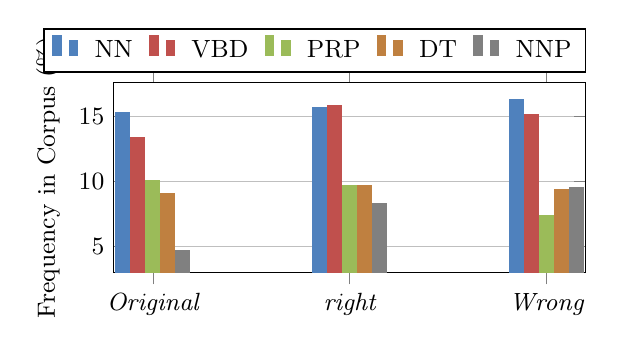
\begin{tikzpicture}
\small
    \begin{axis}[
        width  = 0.4*\textwidth,
        height = 4cm,
      %  major x tick style = transparent,
        ybar=\pgflinewidth,
        x=2.5cm,
       bar width=5pt,
        ymajorgrids = true,
        ylabel = {Frequency in Corpus (\%)},
        symbolic x coords={{\it Original}, {\it right}, {\it Wrong}},
        xtick = data,
        scaled y ticks = false,
        %enlarge x limits=0.25,
        ymin=3,
        legend cell align=left,
        legend style={
        		legend columns=-1,
                at={(1,1.05)},
                anchor=south east,
                column sep=1ex
        }
    ]
        \addplot[style={bblue,fill=bblue,mark=none}]
            coordinates {({\it Original}, 15.3) ({\it right}, 15.7) ({\it Wrong}, 16.3)};

        \addplot[style={rred,fill=rred,mark=none}]
            coordinates {({\it Original}, 13.4) ({\it right}, 15.8) ({\it Wrong}, 15.1)};

        \addplot[style={ggreen,fill=ggreen,mark=none}]
            coordinates {({\it Original}, 10.1) ({\it right}, 9.7) ({\it Wrong}, 7.4)};

        \addplot[style={brown,fill=brown,mark=none}]
            coordinates {({\it Original}, 9.1) ({\it right}, 9.7) ({\it Wrong}, 9.4)};

        \addplot[style={gray,fill=gray,mark=none}]
            coordinates {({\it Original}, 4.7) ({\it right}, 8.3) ({\it Wrong}, 9.5)};

        \legend{NN, VBD, PRP, DT, NNP}
    \end{axis}
\end{tikzpicture}
\caption{\label{roc_pos_distribution}PoS tags}
\end{subfigure}
\begin{subfigure}{.5\textwidth}
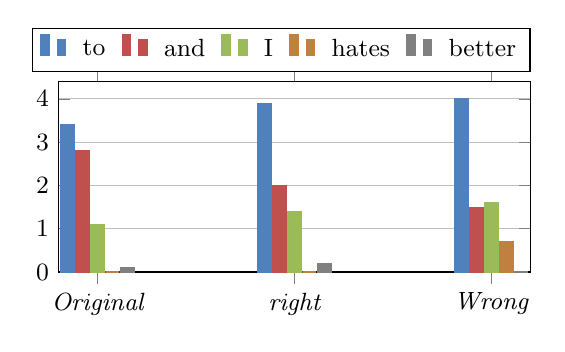
\begin{tikzpicture}
\small
    \begin{axis}[
        width  = 0.4*\textwidth,
        height = 4cm,
      %  major x tick style = transparent,
        ybar=\pgflinewidth,
        x=2.5cm,
       bar width=5pt,
        ymajorgrids = true,
%        ylabel = {Frequency in Corpus (\%)},
        symbolic x coords={{\it Original}, {\it right}, {\it Wrong}},
        xtick = data,
        scaled y ticks = false,
        %enlarge x limits=0.25,
        ymin=0,
        legend cell align=left,
        legend style={
        		legend columns=-1,
                at={(1,1.05)},
                anchor=south east,
                column sep=1ex
        }
    ]
        \addplot[style={bblue,fill=bblue,mark=none}]
            coordinates {({\it Original}, 3.4) ({\it right}, 3.9) ({\it Wrong}, 4)};

        \addplot[style={rred,fill=rred,mark=none}]
            coordinates {({\it Original}, 2.8) ({\it right}, 2) ({\it Wrong}, 1.5)};

        \addplot[style={ggreen,fill=ggreen,mark=none}]
            coordinates {({\it Original}, 1.1) ({\it right}, 1.4) ({\it Wrong}, 1.6)};

        \addplot[style={brown,fill=brown,mark=none}]
            coordinates {({\it Original}, 0) ({\it right}, 0) ({\it Wrong}, 0.7)};

        \addplot[style={gray,fill=gray,mark=none}]
            coordinates {({\it Original}, 0.1) ({\it right}, 0.2) ({\it Wrong}, 0)};

        \legend{to, and, I, hates, better}
    \end{axis}
\end{tikzpicture}
\caption{\label{roc_word_distribution}Words}
\end{subfigure}
\caption{The distribution of five frequent POS tags (\ref{roc_pos_distribution}) and words (\ref{roc_word_distribution})  across different endings: {\it Original} -- endings of stories from the ROC story corpus (the story cloze training set). {\it right} -- correct endings, {\it Wrong} -- wrong endings (both from story cloze task).}

\end{figure*}


%\roy{Other things to talk about (not necessarily in that order): 
%1. no training corpus for the task. That is, the training set (a) does not contain negative example (just positive), and (b) was not generated in the same way as the positive test samples. Here you need to explicitly say that we show that we show that the training and test sets use very different styles.
%2. Maybe talk about the shared task, as well as their RepEval paper, which suggested this task as a vector-space evaluation measure?
%3. Say that the authors did an extensive work in order to  assure that the positive and negative samples are not easily distinguishable: for each pair, both endings were written by the same author (you addressed this earlier, but this seems like a better location), they tried an extensive set of baselines, showing all don't surpass a random baseline by much. Maybe now you can briefly mention the benchmarks, saying that several baselines were presented in the papers. All benchmarks attempted to learn the connection between the previous paragraph and the ending, and all performed near chance level.. However, no baseline looked at the endings independently. 
%Then you can add the benchmark text below, and conclude that this indicates that this task is well designed and hard and the one hand, but might also point to potential disagreements between the train and the test data, which we highlight in this paper.}


\isectionb{Model}

The goal of this paper is to determine the extent to which 
%does constraining authors in their writing assignments lead to them adopting different writing styles. 
different writing constraints lead the authors to adopt different writing styles. 
In order to answer these questions, we use simple, classic NLP tools, which have been shown to be very effective for recognizing style (see \secref{Related}).
We describe our model below.

We train a linear logistic regression (aka Maximum Entropy) classifier to distinguish between different endings. 
Each feature vector is computed using the words in one ending, without considering earlier parts of the story. 
We use the following style features.

\begin{itemize}
\item\textit{\textbf{Length}.} The number of words in the sentence.
\item\textit{\textbf{Word n-grams.}} We use sequences of 1-5 words. Following \cite{Tsur:2010,Schwartz:2013}, we distinguish between high frequency and low frequency words. 
Specifically, we replace content words, which are often low frequency, with their part-of-speech tags (Nouns, Verbs, Adjectives and Adverbs).
\item\textit{\textbf{Character n-grams.}} Character n-grams are one of the most useful features in identifying author style \cite{Stamatatos:2009}. 
We use character 4-grams.
\end{itemize}

\isectionb{Experiments}
We design two experiments to answer our research questions. 
The first is an attempt to distinguish between the {\it right} and {\it wrong} endings.
The second attempts to distinguish between the {\it original} endings and new ({\it right}) endings.
We describe both experiments below.

\paragraph{Experiment 1: Correct/Wrong Endings.}
The goal of this experiment is to measure to what extent  style features capture differences between the {\it right} and {\it wrong} endings.
As the cloze story task doesn't have a training corpus for the {\it right} and {\it wrong} endings (see \secref{ROC_Story}), we use the development set as our training set. 
We split it (90/10) into our training and development set. We keep the story cloze test set as is.
The final size of our training/development/test sizes are 3,366/374/3,742 endings, respectively. 

It is worth nothing that our classification task is slightly different from the { story cloze task}. 
Instead of classifying pairs of endings, one which is {\it right} and another which is {\it wrong}, we take the set of  {\it right} endings as positive samples and the set of {\it wrong} endings as our negative examples. 
By ignoring the coupling between {\it right} and {\it wrong} pairs, we are able make a more general claim about the style used when writing each of the tasks.

\paragraph{Experiment 2: Original/New Endings.}

Here the goal is to measure whether writing the ending as part of a story imposes different style compared to writing a ({\it right}) ending to an existing story.
We use the endings of the ROC stories as our {\it original} training samples and {\it right} endings from the story cloze task  development and test sets as {\it new} training samples.
As there are far more {\it original} samples than {\it new} ones, we randomly select $N$ {\it original} samples, where $N$ is the number of {\it new} samples,
such that we have balanced labels in our training, validation and test sets (sizes are the same as in Experiment 1).
We randomly sample 5 training sets and report the average classification result.

\paragraph{Experimental Setup.}
In both experiments, we add a START symbol at the beginning of each sentence.\footnote{Virtually all sentences end with a period or an exclamation mark, so we do not add an END token} 
For computing our features, we keep n-gram (character or word) features that occur at least five times in the training set.
All feature values are normalized to [0-1].
For the POS features, we tag all endings with the Spacy POS tagger.\footnote{\url{spacy.io/}}
We use  python's sklearn logistic regression implementation with L2 loss. 
We grid search the regularization parameter on our development set. 


\isectionb{Results}
\figref{results} shows our results.
Results show that for Experiment 1, our model obtains results well above a random baseline -- 64.5\% classification accuracy. 
For Experiment 2, we get even higher results -- 68.5\%. 
These numbers indicate that these different writing tasks clearly impose different writing styles on authors. 

As a complementary experiment, we measured whether these style differences are additive. 
That is, whether the style differences between {\it right} endings and {\it wrong} ones are different from the differences between {\it right} and {\it original} endings.
We repeated Experiment 2, this time comparing between {\it original} and {\it wrong} sentences. 
Our hypothesis is that differences would be even clearer. 
Our results (\figref{results}) show that this is indeed the case: the classifier's accuracy jumps to 75.2\%.

\begin{figure}
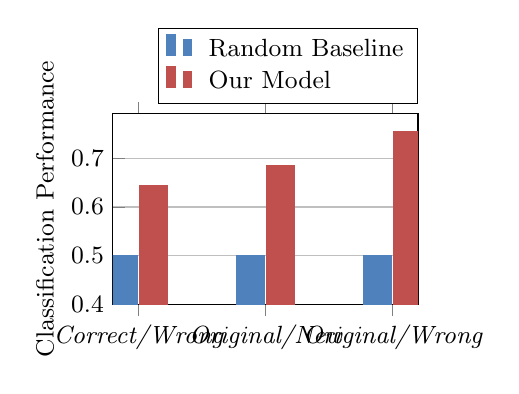
\begin{tikzpicture}
\small
    \begin{axis}[
        width  = 0.45*\textwidth,
        height = 4cm,
      %  major x tick style = transparent,
        ybar=2*\pgflinewidth,
       % bar width=14pt,
        ymajorgrids = true,
        ylabel = {Classification Performance},
        symbolic x coords={{\it Correct/Wrong}, {\it Original/New}, {\it Original/Wrong}},
        xtick = data,
        scaled y ticks = false,
        %enlarge x limits=0.25,
        ymin=0.4,
        legend cell align=left,
        legend style={
                at={(1,1.05)},
                anchor=south east,
                column sep=1ex
        }
    ]
        \addplot[style={bblue,fill=bblue,mark=none}]
            coordinates {({\it Correct/Wrong}, 0.5) ({\it Original/New}, 0.5) ({\it Original/Wrong},.5)};

        \addplot[style={rred,fill=rred,mark=none}]
            coordinates {({\it Correct/Wrong}, 0.645) ({\it Original/New}, 0.685) ({\it Original/Wrong},0.756)};

        \legend{Random Baseline, Our Model}
    \end{axis}
\end{tikzpicture}
\caption{\label{results} Results of  experiments 1 and 2 (left two charts). 
Rightmost graph shows a control experiment which classifies {\it original} endings vs \textit{\textbf{wrong}} endings. }
\end{figure}


\paragraph{Story Cloze Task.}
The results of Experiment 1 indicate that {\it right} and {\it wrong} endings are characterized by different styles.
In order to further estimate the quality of our classification results, we tackle the story cloze task using our classifier.
This classification task is more constrained than Experiment 1, as here the task is given two endings, which one is {\it right} and which is {\it wrong}.
In order to solve the task, we use the output of our trained classifier. 
For each pair of endings in our test set, if the classifier assigns different labels to them, we keep these labels. 
If they share the same label, then one of them must be wrong, so we use the classifier confidence level as a deciding factor: the label of the one with the lower confidence is reversed. 

\tabref{cloze_results} shows our results on the story cloze test set. Our classifier obtains 72.4\% accuracy, which is 12.5\% higher than the published state-of-the-art result on the task.
Importantly, unlike previous approaches, our classifier does not require the story corpus training data, and in fact doesn't even look at the first four sentences of the story in question.
These numbers indicate that the styles of {\it right} and {\it wrong} endings are indeed very different.

Other than the published works that tackled this task, a few  recent works published their results in the LSDSem shared task website.\footnote{\url{https://competitions.codalab.org/competitions/15333}} 
At the time of submission, our results are still state-of-the-art (though by a  smaller margin). 
No other information other than the name of the groups and their results is available.

\begin{table}[!t]
\begin{center}
%\small
\begin{tabular}{|c|c|} \hline
{\bf Model} & {\bf Results} \\ \hline
{DSSM} \cite{Mostafazadeh:2016} & 0.585 \\ \hline
{ LexVec} \cite{Salle:2016} & 0.599 \\ \hline\hline
{ Niko (shared task)}	& 0.7\\ \hline
{ tbmihaylov (shared task)} & 0.711\\ \hline\hline
{RNN}		& 0.677 \\ \hline
{\bf Our Model} & {\bf 0.724} \\ \hline
{\bf Combined (Our model, RNN)} & {\bf 0.752} \\ \hline\hline
Human judgment & 1 \\ \hline
\end{tabular}
\end{center}
\caption{\label{cloze_results}
Results on the test set of the cloze story task. 
Upper part are published results.
LexVec results are taken from \cite{Speer:2016}.
Results in the middle part are taken from the LSDSem 2017 shared task webpage.
Bottom part is our results.
RNN is our implementation of an RNN.
}
\end{table}


\paragraph{Combination with an RLM.}
We investigate whether our model can benefit from state-of-the-art text comprehension models, for which this task was designed. 
Specifically, we experiment with a recurrent language model (RLM, \citet{mikolov2010recurrent}). % on the ROC story corpus training data,
%and use it to compute the probability of both {\it right} and {\it wrong} endings in the story cloze test set.
Unlike the model in this paper, which only considers the story endings, this language model follows the protocol suggested by the story cloze task designers, and harnesses the ROC Stories training set, which consists of single-ending stories. 
We show that adding the language model features  further boosts our performance on the story cloze task.


We train the RLM using a single-layer LSTM \cite{hochreiter1997long} of hidden dimension $h=512$.
We use the ROC Stories for training, setting aside $10\%$ for validation of the language model. 
We replace all words occurring less than 3 times by a special out-of-vocabulary character, yielding a vocabulary size of $|V|=$21,582.
Only during training, we apply a dropout rate of 60\% while running the LSTM over all 5 sentences of the stories. 
Using AdamOptimizer \cite{kingma2014adam} and a learning rate of $\eta=.001$, we train with backpropagation on cross-entropy. % minibatches of $50$ stories.
% h=512, dropout rate of 60%, V=21582, 10% validation set


% Eval
On its own, our neural language model performs moderately on the story cloze test. 
This is not surprising, as \citet{Mostafazadeh:2016} hinted  that simple language models do not perform well on the task. 
Indeed, using our neural LM and selecting endings based on $p_\theta(ending|story)$, we obtain only $55\%$ accuracy. 
However, when using the likelihood ratio $\frac{p_\theta(ending|story)}{p_\theta(ending)}$ to select endings, performance jumps to $67.7\%$ (see \tabref{cloze_results}).\footnote{Further analysis of this large performance gain is out of the scope of this paper.}

We combine our linear model with the RLM by adding three features to our classifier: $p_\theta(ending|story),p_\theta(ending)$ and $\frac{p_\theta(ending|story)}{p_\theta(ending)}$. 
We retrain our linear  model with the new feature set, and gain a performance   boost  of $2.8\%$ -- up to 75.2\%, which is 15.3\% better than the published state-of-the-art, and 4.1\% better than the best unpublished result.
These results indicate that while style features can be used to obtain high accuracy on the task, adding context and training on a large dataset can improve performance even more.




\isection{Ablation Study}{Ablation}



\paragraph{Most Discriminative Feature Types.}
A natural question that follows this study is which features are most helpful in making predictions about writing style. 
To answer this question, we re-ran Experiment 1 with different sub-groups of features. 
\tabref{subgroups} shows our results. Results clearly show that  character n-grams are the most effective style predictors, reaching within  0.6\% of the full model, but that word n-grams also capture much of the signal, yielding 61.2\%. 
These findings are in line with previous works that used character n-grams along with other types of features to predict writing  style \cite{Schwartz:2013}.


\begin{table}[!t]
\begin{center}
%\small
\begin{tabular}{|c|c|} \hline
{\bf Feature Type} & {\bf Result}\\ \hline
Word n-grams & 61.2\% \\ \hline
Char n-grams & 63.9\% \\ \hline
Full Model & 64.5\% \\ \hline

\end{tabular}
\end{center}
\caption{\label{subgroups}
Results on Experiment 1 with different types of features.
}
\end{table}

\paragraph{Most Salient Features -- Experiment 1.}
%In order to understand which features were most salient, we repeated Experiment 1, this time running SVM with L1 norm, such that it generates a sparse separating hyperplane. 
%This came at a minor cost of less than 2\% in performance compared to our L2 results (0.697 compared to 0.724).  
\tabref{exp1_features} shows the five features with the highest positive and negative weights in the logistic regression classifier hyperplane for Experiment 1. 
These correspond to the 5 most salient features for {\it right} (coherent) and {\it wrong} (incoherent) endings, respectively.

The table shows a few interesting trends. 
First, authors tend to structure their sentences differently when writing {coherent}  vs. {incoherent} endings.
For instance, {coherent} endings are more likely to start with an adverb (e.g., ``then'', ``so'', ``eventually''), while {incoherent} ones tend to start with a proper noun.
In addition, we find that {incoherent} endings are more likely to finish the sentence with a common noun. 

More interestingly, the different writing tasks seem to impose a specific sentiment on the writer. 
Three of the top four most salient features for detecting {\it wrong} endings are variants of the verb ``hate''.
This indicates that when authors are asked to write {\it wrong} text, they tend to use negative language.

An alternative explanation to this hypothesis might be that the first four sentences of the stories in the ROC story corpus tend to be positive, and thus in order to make an ending {\it wrong}, authors adopted a negative approach. 
A similar idea was suggested in the original story cloze paper, where two sentiment-based baselines were evaluated. 
These baselines measured the relative sentiment between the ending and the previous sentences.
The performance of both these baselines was roughly chance-level, which seems to suggest that this is not the case.
\yc{Is it really because there's no statistical tendency in the original stories to have happy endings, as opposed to the alternative possibility --- the sentiment classifier used by Monstafazadeh 2016 didn't quite nail down the optimal feature encodings?} 

\begin{table}[!t]
\begin{center}
%\small
\begin{tabular}{|c|c|} \hline
\textit{\textbf{Correct}} & \textit{\textbf{Wrong}}\\ \hline
`ally' & ` hate'\\ \hline
`VBD the' & ` hat'\\ \hline
`START RB' & `START NNP'\\ \hline
`ved ' & `ated'\\ \hline
` tim' & `NN .'\\ \hline

\end{tabular}
\end{center}
\caption{\label{exp1_features}}
The top 5 most discriminative features for predicting {\it right} and {\it wrong} endings.\end{table}


\paragraph{Most Salient Features -- Experiment 2.}
%In order to understand which features were most salient, we repeated Experiment 1, this time running SVM with L1 norm, such that it generates a sparse separating hyperplane. 
%This came at a minor cost of less than 2\% in performance compared to our L2 results (0.697 compared to 0.724).  
\tabref{exp2_features} shows the same analysis for Experiment 2.
Interestingly, here the most salient features are quite different. 
As noticed on \secref{ROC_Story}, {\it original} endings tend to be much longer, which is indeed the most salient feature for them.
Another clear style difference is the use of punctuation: {\it original} endings often end with exclamation marks, while {\it new} endings end almost exclusively with periods. 
Finally, syntactic difference appear to play an important role in stylistic differences between the two tasks. 
Specifically, {\it original} endings contain more common nouns (NN), adverbs (RB) and gerunds (VBG), while {\it new} endings seem to contain more past tense verbs (VBD), especially as the second word in the sentence.


\begin{table}[!t]
\begin{center}
%\small
\begin{tabular}{|c|c|} \hline
\textit{\textbf{Original}} & \textit{\textbf{New}}\\ \hline
{\it length} & `.'\\ \hline
`!' & `START NNP'\\ \hline
`NN' & `START NNP VBD'\\ \hline
`RB' & `START I VBD'\\ \hline
`VBG' & `NNS .'\\ \hline

\end{tabular}
\end{center}
\caption{\label{exp2_features}}
The top 5 most discriminative features for predicting {\it original} and {\it new} ({\it right}) endings.\end{table}


\isectionb{Discussion}

In this paper we have shown that different writing tasks affect writing style. 
Our results indicate that when authors are asked to write the last sentence of a five sentence story, they will use different style to write a {\it right} ending compared to a {\it wrong} ending. We have also shown that writing the ending as part of a five sentence story is very different than reading four sentences and then writing the fifth.

Our findings hint that the nature of the writing task imposes a different mental state on the author, which is expressed in ways which are often implicit, but can be unfolded using simple automatic tools. 
This is in line with previous cognitive findings. 
For instance, previous studies have shown that when answering questions, people  tend to adopt the writing style of the question \cite{Ireland:2010}.


Other studies have shown that writing tasks can even have a long term effect.
A range of works have shown that writing emotional texts and benefit both physical and mental health \cite{Lepore:2002,Frattaroli:2006}. 
Some of these works showed that these changes are also accompanied by changes in writing style \cite{Campbell:2003}. 
The results of the current study can shed more light on the processes that people undergo when presented with different writing tasks.


This paper also reveals several important lessons for the future design of NLP tasks. 
First, it stresses the need to carefully control for even seemingly minor details. 
Second, it emphasizes the importance of running baseline models.
While recent advances in NLP  suggest that many classic NLP methods are out-of-date, 
this is not necessarily the case, especially for small datasets.
This is particularly important in order to ensure that  new technological improvements are capturing a qualitatively different signal.
Luckily, the substantial improvement we get when combining our model with the RNN language model (\secref{Experiments}) suggests that despite the high results obtained by the simple, classic model, the more recent RNN approach captures a different aspect of the task.

\isection{Related Work}{Related}

\paragraph{Writing Style.}
Writing style has been an active topic of research for decades now. 
The models used to effectively solve  such tasks are often linear classifiers with style features such as character and word n-grams \cite{Stamatatos:2009,Koppel:2009}.
Previous works have shown that different authors can be grouped by their writing style, according to factors such as age \cite{Pennebaker:2003,Argamon:2003,Schler:2006,Rosenthal:2011}, gender \cite{Argamon:2003,Schler:2006} and native language \cite{Koppel:2005}.
At the extreme case, each individual author adopts a unique writing style \cite{pennebaker1999linguistic,Schwartz:2013}. 
Interestingly, previous work have shown that individual style can be affected from coarse-grained factors such as those just described, but also from other less apparent factors such as mental state, or even living in a high elevation location \cite{schwartz2013personality}.

Unlike the works just described which compare the writing style between different authors, some works have shown that the same author can adopt different style used when writing positive vs. negative text \cite{Davidov:2010} and when writing sarcastic text \cite{Tsur:2010}. In this work, we have shown that the same author can adopt a different style when facing different writing tasks.

The line of works that most resembles our work is the detection of deceptive text. 
Several works used stylometric features to  predict deception 
\cite{Newman:2003,hancock2007lying,ott2011finding,Feng:2012}.
Some works even showed that writing style applied when lying is different across genders \cite{Perez:2014a,Perez:2014b}.
In this work, we have shown that an even more subtle writing task -- writing {\it coherent} and {\it incoherent} story endings -- imposes different styles on the author.


\paragraph{Machine Reading.}
The cloze story task, which is the focus of this paper, is part of a wide set of machine reading works published in the last couple of years.
These include datasets like bAbI \cite{Weston:2015}, SNLI \cite{bowman2015large}, CNN/DailyMail \cite{hermann2015teaching}, SQuAD \cite{rajpurkar2016squad} and LAMBADA \cite{Paperno:2016}. 

While these works have presented valuable resources for the NLP community (as well as for the deep learning community), 
it is often the case that these datasets suffer from methodological problems, such as inherent ambiguity caused by applying automatic tools when generating the datasets \cite{Chen:2016}. 
In this paper we have pointed to other methodological problems in  machine reading tasks, namely the different writing tasks used to generated the data, which largely affect the writing style of the positive and negative samples, as well as create a discrepancy between the training and the test data.


\isectionb{Conclusion}

The research question that guided this work is the extent to which different writing tasks result in different writing styles.
We experimented with the story cloze task, which introduces two interesting comparison points: %setups for our purposes:
%a setup where the same author writes both a {\it right} and an {\it wrong} ending to a story, 
%and one which compares an ending written as part of a story to a standalone ending added to a story written by someone else.
 the difference between people writing a story on their own and people continuing someone else's story 
 and the difference between the same author writing a coherent and an incoherent story ending.
In both cases, a simple linear model reveals measurable differences in people's writing styles, %that different styles are imposed.
%The different styles allow our style detection 
which in turn allows our final 
model to reach state-of-the-art results on the story cloze task, more than 12\% improvement compared to the best published result.

The findings presented in this paper have  cognitive implications, as they motivate further research on the exact effect that different writing tasks have on humans.
They also provide valuable lessons for designing new NLP datasets.
Future work will include testing whether other similar writing tasks, such as fake news, also impose their own unique and identifiable style on their authors.




% include your own bib file like this:
%\bibliographystyle{acl}
%\bibliography{acl2017}

\newpage
\bibliography{acl2017}
\bibliographystyle{acl_natbib}

\end{document}
